\chapter{ Elettrostatica nel Vuoto}

\section{Introduzione all'Elettrostatica}
La prima cosa che dobbiamo andare a definire all'interno del corso è il concetto di \textbf{forza}. Ogni interazione ha origine nella materia, ne esistono di diverse che vanno a generare tutte le forze di cui oggigiorno siamo a conoscenza:

\begin{itemize}
	\item Forza di Gravità $\rightarrow$ $\vec{F_g}$
	\item \textbf{Forza Elettromotrice} $\rightarrow$ $\vec{F}_{em}$
	\item Forze Nucleari Deboli e Forti 
\end{itemize}

Mentre la forza di gravità e elettro motrice sono forze a lungo raggio, quelle nucleari sono forze a corto raggio che agiscono nel campo microscopico. Per quanto riguarda le forze a lungo raggio, si tratta di forze le cui interazioni sono osservabili anche all'infinito

\subsection{Fatti Sperimentali}
Si può osservare tramite degli esperimenti che esiste una interazione tra corpi che non è descrivibile tramite la meccanica classica: avvicinando corpi dotati di \textbf{carica elettrica}, che può essere positiva o negativa, sperimentiamo \textbf{forze attrattive} o \textbf{repulsive}.

In generale abbiamo che cariche dello stesso segno si respingono, mentre cariche discordi si attraggono. Indicheremo le cariche con il simbolo $q$. 
\begin{figure}[ht]
	\begin{center}
		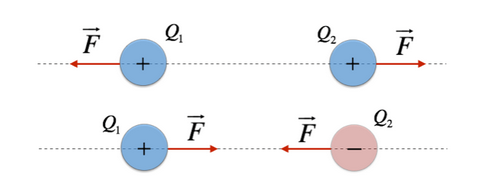
\includegraphics[width=0.5\textwidth]{./Media/Coulomb.png}
		\caption{Attrazione e Repulsione di Cariche}
	\end{center}
\end{figure}

Se la massa ha la proprietà di essere unicamente positiva, la carica può essere sia positiva che negativa, proprio per questo motivo la forza di gravità è soltanto attrattiva, mentre l'interazione che stiamo introducendo può essere sia attrattiva che repulsiva.

A livello microscopico abbiamo a disposizione tre diversi strumenti per \textbf{indurre carica}  all'interno della materia: 

\begin{itemize}
	\item strofinio
	\item induzione
	\item contatto
\end{itemize}

Sappiamo che un \textbf{atomo} si compone di un \textit{nucleo} contenente \textit{neutroni} e \textit{protoni}, attorno a tale nucleo abbiamo una \textit{nuvola elettronica} di particelle elementari a carica negativa. Si osserva che ogni quantità di carica che troviamo in natura è un \textit{multiplo della carica dell'elettrone}. Per questo motivo la carica dell'elettrone si dice \textbf{carica elementare}.

Ordinariamente la materia che troviamo in natura è \textbf{neutra}, ovvero il numero di elettroni e protoni è lo stesso. 

\subsection{Elettrizzazione per Strofinio}
Nel momento in cui vado a strofinare un oggetto, a livello meccanico vengono spostati degli elettroni da un corpo all'altro. Per mezzo di questa procedura, il corpo che cede elettroni, diventerà carico positivamente, l'altro sarà carico negativamente. 

Entrambi i due materiali ora elettrizzati avranno la \textbf{stessa quantità di carica} di segno chiaramente opposto. Un'altra considerazione che viene abbastanza naturale fare, è che la quantità di carica al termine dell'esperimento la quantità di carica si conserva e rimane neutra.

\medskip


\begin{tcolorbox}
	\begin{center}
				In un sistema isolato, la $Q_{tot}$ si \textbf{conserva}
			\end{center}
\end{tcolorbox}


Chiaramente quale oggetto ceda elettroni all'altro dipende dalle caratteristiche dei materiali di cui si compongono gli oggetti.

\subsection{Elettrizzazione per Induzione}
Nel momento in cui vado ad \textit{avvicinare} un oggetto con una certa carica ad un oggetto neutro, le cariche di segno opposto nell'oggetto neutro verranno attratte in prossimità dell'oggetto carico, mentre le cariche di segno uguale verranno respinte all'estremità opposta dell'oggetto

\begin{figure}[ht]
	\begin{center}
		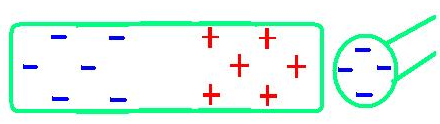
\includegraphics[width=0.5\textwidth]{./Media/Induzione.png}
		\caption{Elettrizzazione per Induzione}
	\end{center}
\end{figure}

Nel momento in cui viene spostato il materiale che subisce induzione, l'azione della carica induttrice sarà maggiore o minore a seconda della distanza, ciò si può sperimentare per mezzo di un \textbf{elettroscopio}.  Tramite un esperimento con l'elettroscopio è possibile dedurre il seguente fatto: 

\begin{tcolorbox}
	\begin{center}
		In elettrostatica vale il \textbf{principio di sovrapposizione}, ovvero le azioni delle cariche si sovrappongono nella forza elettrostatica. Ciò verrà dimostrato in seguito.
	\end{center}
\end{tcolorbox}


\subsection{Elettrizzazione per Contatto}
Nel momento in cui metto a contatto un oggetto carico con un altro materiale neutro, otteniamo dal punto di vista fisico, un unico oggetto carico (che chiameremo \textbf{conduttore}). Se prendo un conduttore carico e lo \textit{collego alla Terra} le cariche possono migrare, dato che il conduttore diventa un tutt'uno con la terra. 

\subsection{Natura dei Materiali}
I materiali tendono a comportarsi in due modi differenti, tali comportamenti vanno a caratterizzare due tipologie di materiali: 

\begin{description}
	\item[Conduttori] sono materiali che si compongono di \textit{cariche libere di muoversi}. Si tratta di tutti quei materiali che una volta spostati da un materiale carico ritornano allo stato precedente.
	\item[Dielettrici] sono materiali nei quali gli \textit{elettroni sono vincolati agli atomi}. Nel momento in cui viene avvicinato un materiale carico ad un dielettrico avverrà spostamento di carica (così come anche per i conduttori) ma all'interno del materiale i \textit{centri di simmetria delle cariche} smettono di coincidere
\end{description}

\section{Forza Elettrostatica e Legge di Coulomb}

Come suggerisce la parola \textit{statica} non andremo, per ora, a considerare variazioni nel tempo. Questo porta il vantaggio di riuscire a studiare il campo elettrico e quello magnetico in maniera separata, contrariamente a quanto accade in elettrodinamica. 

\subsection{Fatti Sperimentali}
Per sperimentare l'interazione elettrica tra due cariche (concordi o discordi) si utilizza una \textbf{bilancia di torsione}

\medskip

\begin{figure} [ht]
	\centering
	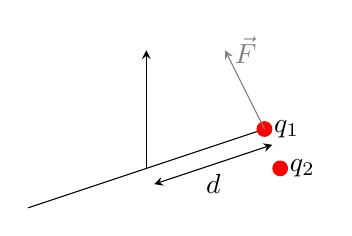
\begin{tikzpicture}
		\draw (0,0) -- (3,1);
		\draw[-stealth] (1.5, 0.5) -- (1.5, 2);
		\draw[stealth-stealth] (1.6, 0.3) -- (3.1, 0.8) node [midway, below] {$d$};
		\fill[red] (3,1) circle  [radius=0.1] node [color=black, right] {$q_1$};
		\fill[red] (3.2,0.5) circle [radius=0.1] node [color=black, right] {$q_2$};
		
		\draw[color=black!50, -stealth] (3,1) -- (2.5,2) node [right] {$\vec{F}$};
	\end{tikzpicture}
	\caption{Bilancia di Torsione}
\end{figure}

Si osserva che, data $r$ la distanza tra le due cariche, otteniamo che $|\vec{F_{el}}| = K\frac{q_1q_2}{r^2}$, e valorizzando il coefficiente $K$ troviamo la seguente equazione dell'\textbf{interazione di Coulomb}: 

\begin{large}
\begin{equation}
	|\vec{F}| = \frac{1}{4\pi\epsilon_0} \frac{q_1q_2}{r_{12}^2} \hat{r}
	\label{f_coulomb}
\end{equation}
\end{large}


Tale forza va ad agire \textit{sulla particella $q_1$} , prende la direzione del vettore distanza tra $q_1$ e $q_2$ e si misura, ovviamente, in \textbf{Newton}; per quanto riguarda invece l'unità di misura della carica abbiamo $[q] = C$ (\textbf{Coulomb}). Il valore $\epsilon_0$ è detta \textbf{costante dielettrica del vuoto}

Chiaramente vale la \textbf{terza legge di Newton}, che dice che per ogni forza da una particella $q_1$ a una particella $q_2$, ne agisce una uguale e contraria da $q_2$ a $q_1$ . Si osserva che il prodotto delle due cariche va a caratterizzare la \textit{attrattività} o la \textit{repulsività} del fenomeno in questione infatti: 

\begin{itemize}
	\item $sgn(q_1) = sgn(q_2)$: le forze seguono le direzioni dei versori, dunque abbiamo un'azione \textbf{repulsiva}
	\item $sgn(q_1)  \neq sgn(q_2)$: il verso delle forze si ribalta e otteniamo una azione \textbf{attrattiva}
\end{itemize}

\subsection{Generalizzazione a un sistema di n cariche}

\begin{figure} [ht]
	\centering
	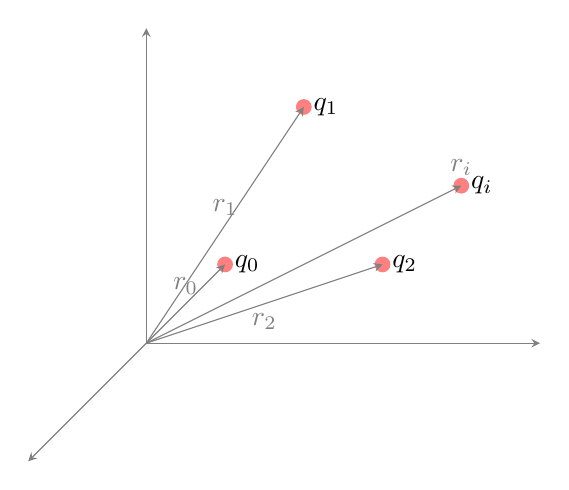
\begin{tikzpicture}
		% assi cartesiani
		\draw[color=black!50, -stealth] (0,0) -- (5,0);
		\draw[color=black!50, -stealth]  (0,0) -- (0,4);
		\draw[color=black!50, -stealth] (0,0) -- (-1.5,-1.5);
		
		% n cariche
		\fill[color=red!50] (1,1) circle (0.1) node [color=black, right] {$q_0$};
		\fill[color=red!50] (2,3) circle (0.1) node [color=black, right] {$q_1$};
		\fill[color=red!50] (3,1) circle (0.1) node [color=black, right] {$q_2$};
		\fill[color=red!50] (4,2) circle (0.1) node [color=black, right] {$q_i$};
		
		% raggi vettore
		\draw[color=gray, -stealth] (0,0) -- (1,1) node[midway, above] {$r_0$};
		\draw[color=gray, -stealth] (0,0) -- (2,3) node[midway, above] {$r_1$};
		\draw[color=gray, -stealth] (0,0) -- (3,1) node[midway, below] {$r_2$};
		\draw[color=gray, -stealth] (0,0) -- (4,2) node[right, above] {$r_i$};
		
	\end{tikzpicture}
	\caption{Sistema discreto di $n$ cariche}
	\label{sistema_n_cariche}
\end{figure}

In un sistema come quello di cui sopra, vale il \textbf{principio di sovrapposizione}, ciò implica l'importante concetto di \textit{indipendenza dei fenomeni}. Sulla generica particella $q_0$ agirà la seguente forza  risultate: 

\begin{equation}
	\sum_{i = 1}^{n}  \frac{q_i q_0}{4\pi\epsilon_0} \frac{\hat{r}_{i0}}{r_{i0}^2}
	\label{f_coulomb_sistema}
\end{equation}

\section{Campo Elettrostatico}
La prima domanda che può sorgere è il \textit{perché} serva introdurre il concetto di \textbf{campo elettrostatico}.  Il motivo è che ipotizzando di spostare una carica all'interno del sistema \ref{sistema_n_cariche}, stando alle leggi descritte nell'equazione \ref{f_coulomb_sistema}, dato che varia il sistema, andrò a misurare una forza differente, tale variazione avviene però in modo \textbf{istantaneo}. 

Questo non è possibile, dato che la massima velocità di trasmissione di informazione è quella della luce; questa visione porta dunque alla contraddizione dell'\textbf{azione istantanea} che in fisica non esiste.

Come già anticipato, risolviamo questo importante vincolo tramite il concetto di \textbf{campo elettrostatico}, infatti osservando attentamente l'equazione \ref{f_coulomb_sistema} vediamo che la forza è \textit{proporzionale a $q_0$} , possiamo dunque scriverla nel seguente modo:

\begin{large}
	\begin{equation}
		\vec{F}_{el} = q_0 \vec{E_i}(\vec{r}_0)
	\end{equation}
\end{large}


Possiamo quindi definire il \textbf{campo elettrostatico} come: 

\begin{large}
\begin{equation}
		E_i(\vec{r}) = \frac{q}{4\pi\epsilon_0 r_i^2} \hat{r} = \frac{\vec{F}}{q_{int}}
	\label{campo_elettrostatico}
\end{equation}
\end{large}

dove $q$ è una carica qualunque ed r è la distanza dal punto di osservazione a tale carica, dunque andando a introdurre la definizione di campo all'interno di \ref{f_coulomb_sistema} troviamo che

\begin{equation}
	\vec{F}_{tot (q_0)} = q_0 \sum_i \vec{E}_i
\end{equation}

Anche nel caso del campo, vale il \textbf{principio di sovrapposizione} e l'unità di misura del campo elettrostatico è data dal $N/C$ esprimibile anche come rapporto volt su metri $V/m$


\subsection{Energia Elettrostatica} \label{en_elettro}
Andiamo in questa sezione a studiare la \textbf{conservatività della forza elettrostatica}. Sappiamo che una forza si dice conservativa se vale: 

\begin{itemize}
	\item il lavoro $L$ è \textbf{indipendente} dal percorso
	\item $\oint{dL} = 0$
	\item esiste $U$ (\textbf{energia potenziale}) tale che $L_{AB} = - \Delta U$
\end{itemize}

Consideriamo quindi il sistema seguente:

\begin{figure}[ht]
	\centering
	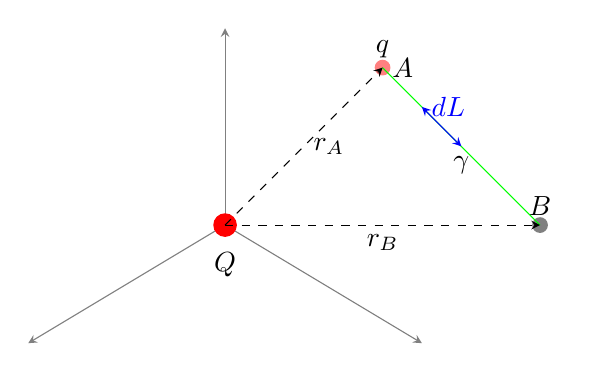
\begin{tikzpicture}
		% assi cartesiani
		\draw[color=black!50, -stealth] (0,0) -- (0,2.5);
		\draw[color=black!50, -stealth] (0,0) -- (-2.5,-1.5);
		\draw[color=black!50, -stealth] (0,0) -- (2.5,-1.5);
		
		\coordinate (A) at (0,-0.5);
		% cairca sorgente
		\fill[color=red] (0,0) circle[radius=0.15] node[color=black]  at (A) {$Q$};
		
		\fill[color=red!50] (2,2) circle[radius=0.1] node[color=black, above] {$q$};
		
		\node[right] (B) at (2,2) {$A$};
		\fill[color=black!50] (4, 0) circle[radius=0.1] node[color=black, above] {$B$};
		
		\draw[color=green] (2,2) -- (4,0) node[color=black, midway, below] {$\gamma$};
		\draw[color=blue, stealth-stealth] (3,1) -- (2.5,1.5) node [right]{$dL$};
		
		\draw[color=black,dashed,  -stealth] (0,0) -- (2,2) node[midway, right] {$r_A$};
		\draw[color=black, dashed, -stealth] (0,0) -- (4,0) node[midway,below] {$r_B$}; 
	\end{tikzpicture}
\end{figure}

Abbiamo che $dL = \vec{F} \cdot \vec{l} $, ovvero $dL = \frac{qQ}{4\pi\epsilon_0 r^2} \hat{r} \cdot d\vec{l} $. E possiamo quindi esprimere il lavoro da $A$ a $B$ come: 

\begin{equation}
 L_{AB} = \int_{A}^{B} dL = \frac{qQ}{4\pi\epsilon_0} \int_{A}^{B} \frac{\hat{r} \cdot d\vec{l}}{r^2}
 \end{equation}
 
 ossia: 
 
\begin{equation}
 L_{AB} = \frac{qQ}{4\pi\epsilon_0}\int_{r_A}^{r_B} {\frac{dr}{r^2}} = \frac{qQ}{4\pi\epsilon_0} \left(\frac{1}{r_A}-\frac{1}{r_B}\right) = -\Delta U
 \end{equation}
 
 Troviamo quindi che l'\textbf{energia elettrostatica} è data da:
 
\begin{large}
 \begin{equation}
 	U = \frac{qQ}{4\pi\epsilon_0r}  + c[J]
 	\label{en_elettro_1}
 \end{equation}
\end{large}

Così come è stata fatta, l'energia non rappresenta altro che un calcolo, se però andiamo a cercarne il significato scopriamo che la \textbf{forza elettrostatica è conservativa}. Ciò, se ad esempio ipotizziamo di trovarci all'infinito, ci permette di porre $U_\infty = 0$, e quindi di esprimere l'energia nel modo seguente: 

\begin{large}
\begin{equation}
	U = \frac{qQ}{4\pi\epsilon_0} = - (U_\infty - U_r) = \Delta U
	\label{en_elettro_2}
\end{equation}
\end{large}

In pratica il la formulazione dell'energia descritta in \ref{en_elettro_1} rappresenta il lavoro svolto dal campo per allontanare una carica verso l'infinito, ovvero per distruggere il sistema. In modo analogo l'equazione \ref{en_elettro_2} rappresenta il \textit{lavoro esterno} necessario a portare una carica in una certa posizione a partire dall'infinito.

\subsection{Linee di Campo}
Si tratta di una rappresentazione che ci consente di farci un'idea sulla forma del campo elettrostatico, hanno le seguenti caratteristiche: 

\begin{itemize}
	\item sono \textit{tangenti} al campo
	\item escono dalle cariche positive
	\item entrano nelle cariche negative
\end{itemize}

Rispetto ad una carica puntiforme, o riconducibile a tale, seguono la direzione \textbf{radiale}. In qualsiasi altra situazione vale il principio di sovrapposizione e la visualizzazione diventa abbastanza difficile da rappresentare. In generale però, tutti i casi che andremo a considerare rimarranno abbastanza semplici. 

\begin{figure}[ht]
	\centering
	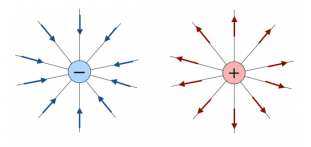
\includegraphics[width=0.7\linewidth]{Media/Linee_Campo}
	\caption{Linee di Campo di una carica puntiforme}
	\label{fig:lineecampo}
\end{figure}


\section{Campo Potenziale Elettrostatico}
 Abbiamo visto come la forza di Coulomb sia colei che va a generare il campo elettrostatico, definito come $\vec{F}/q_{test}$. Abbiamo anche osservato che la forza di Coulomb è conservativa, questo alla luce del fatto che siamo riusciti a ricavarne l'energia potenziale tramite la trattazione descritta in \ref{en_elettro}.
 
 Sappiamo che il campo elettrostatico per una carica puntiforme $q$ , viene percepito ad una distanza $r$ da una particella di test $q_i$ come descritto dall'equazione \ref{campo_elettrostatico}. La forza di Coulomb percepita da tale particella $q_i$ sarà data da $\vec{f} = q_i \vec{E}$ 
 
 Vogliamo capire se possiamo passare ad una visione di \textbf{energia come caratteristica dello spazio}. Si osserva che data una carica unitaria, il campo e la forza coincidono ($E  = F/q_{test}$). Definiamo il \textbf{campo potenziale elettrostatico} come: 
 
 \begin{large}
 \begin{equation}\label{potenziale_elettrostatico}
 	\Delta V_{AB} \equiv \frac{\Delta U_{AB}}{q}
 \end{equation}
\end{large}
 
 Si noti l'analogia con l'equazione \ref{campo_elettrostatico}. In questo caso la $q$ al denominatore è la carica che sto spostando lungo il percorso $AB$. Così come campo elettrostatico e forza elettrostatica coincidono nel caso di cariche unitarie, anche $\Delta V$ e $\Delta U$ coincidono.  Dando un significato fisico a quanto definito fino a qui troviamo che: 
 
 \begin{equation}\label{lavoro_campo_elettrostatico}
 	L = -q \Delta V
 \end{equation} 

Riassumendo dunque, abbiamo che un sistema di cariche sorgenti, va sempre a generare in \textbf{tutto lo spazio} sia un \textbf{campo elettrostatico} $\vec{E}(\vec{r})$ (campo vettoriale) che un \textbf{potenziale elettrostatico} $V(\vec{r})$ (campo scalare). L'unità di misura del potenziale è il \textbf{volt} [$V$]. Da qui dovrebbe risultare chiaro il motivo per cui il campo elettrostatico viene misurato in $V/m$.

\subsection{Calcolo Potenziale Elettrostatico}
Come avevamo $\Delta U = - \int_{A}^{B}{F \cdot dl}$ così abbiamo che: 
\begin{large}
\begin{equation}\label{eq_calcolo_potenziale}
	\Delta V = V_B - V_A = -\int_{A}^{B}\vec{E} \cdot d\vec{l}
\end{equation}
\end{large}

A livello operativo andremo quindi, prima a calcolare il campo $\vec{E}$, in seguito calcolerò l'integrale di cui sopra per il calcolo del potenziale, e a partire da lì mi sarà possibile calcolare tutti quanti i vari lavori. Anche il potenziale verrà definito a meno di una costante. 

Siccome però non vogliamo avere a che fare con una \textbf{differenza di potenziale}, sceglieremo $V(r_0) = V_0$ come valore di riferimento. In molti casi (quando il sistema considerato non è indefinito) potremo scegliere $V(r_0) = V_\infty = 0$. Grazie a queste semplificazioni otterremo: 

\begin{large}
\begin{equation}\label{eq_calcolo_potenziale_2}
	V(r)  = -\int_{r_0}^{r} \vec{E} \cdot d\vec{l}
\end{equation}
\end{large}

Avendo a che fare con integrali di cammino, potremmo chiederci quale cammino scegliere, ma avendo a che fare con una forza conservativa, possiamo sempre scegliere un \textbf{cammino qualunque} (in generale quello \textbf{radiale}). 

\subsection{Superfici Equipotenziali} 
Così come per il campo potremmo chiederci in quale modo rappresentare il potenziale elettrostatico, lo strumento necessario in questo caso diventano le \textbf{superfici equipotenziali}.  Vedremo che il potenziale nel caso di una carica puntiforme alla sorgente in \ref{eq_potenziale_puntiforme}, la cui forma, in punto $r$ qualsiasi per una carica di test è espressa da $V(r) = \frac{Q}{4\pi\epsilon_0 r}$.

Come suggerisce il nome, stiamo cercando le \textit{superfici in cui il potenziale rimane costante}, osservando \ref{lavoro_campo_elettrostatico}, troviamo che $dL = -qdV$ e se voglio $dV = 0$ devo necessariamente avere \textbf{lavoro nullo}. Tale proprietà si raggiunge nel momento in cui $E \cdot ds = 0$ ovvero mi sto spostando in maniera ortogonale al campo. Se voglio avere \textbf{campo perpendicolare alle superfici equipotenziali } devo necessariamente avere come superfici equipotenziali delle \textbf{sfere centrate nella carica sorgente}.

\begin{figure}[ht]
	\centering
	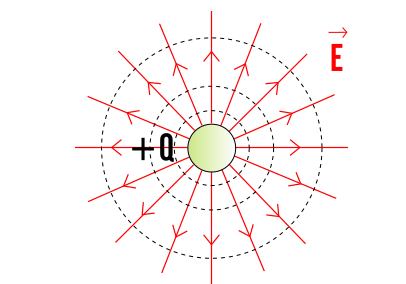
\includegraphics[width=0.7\linewidth]{Media/Sup_Equipotenziali}
	\caption{Superfici Equipotenziali per una carica puntiforme}
	\label{fig:supequipotenziali}
\end{figure}


\section{Relazione Cariche - Campo - Potenziale}
Vogliamo in questa sezione andare a indagare la relazione che viene a crearsi tra cariche sorgenti, campo elettrostatico e potenziale elettrostatico a seconda della configurazione delle cariche sorgenti. 

\subsection{Carica Puntiforme}
Condiserato il seguente sistema di riferimento sappiamo che

\begin{figure}[ht]
	\centering
	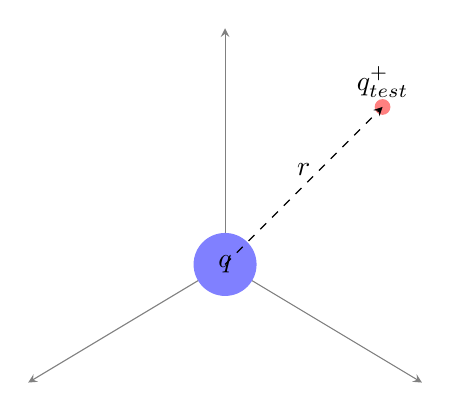
\begin{tikzpicture}
		% assi cartesiani
		
		\draw[color=black!50, -stealth] (0,0) -- (0,3);
		\draw[color=black!50, -stealth] (0,0) -- (-2.5, -1.5);
		\draw[color=black!50, -stealth] (0,0) -- (2.5,-1.5);
		
		% carica puntiforme
		\fill[color=blue!50] (0,0) circle[radius = 0.4]  node[color=black] {$q$};
		%q test
		\fill[color=red!50] (2,2) circle[radius = 0.1]  node[color=black, above] {$q_{test}^+$};
		
		%r
		\draw[dashed, -stealth] (0,0) -- (2,2) node [midway, above] {$r$};
	\end{tikzpicture}
\end{figure}



\begin{equation}
	\vec{E}(r) = \frac{q}{4\pi\epsilon_0 r^2} \hat{r} \longrightarrow V(r)  - V(0)  = -\int_{r_0}^{r} \frac{q}{4\pi\epsilon_0 r^2} \hat{r} \cdot  d\vec{l}
\end{equation}


ma, dato che $\hat{r} \cdot d\vec{l} = dr$ otteniamo semplicemente: 

\begin{equation}
	V(r) - V(0) = - \frac{q}{4 \pi \epsilon_0} \int_{r_0}^{r} \frac{1}{r^2} dr = \frac{q}{4 \pi \epsilon_0}  \left[\frac{1}{r} - \frac{1}{r_0}\right]
\end{equation}

e, ponendo $V_0 = 0$ con $r_0 = \infty$ otteniamo finalmente

\begin{large}
	\begin{equation}\label{eq_potenziale_puntiforme}
		V(r) = \frac{q}{4\pi\epsilon_0r}
	\end{equation}
\end{large}

che è la formula del potenziale per un sistema composto da un'unica \textbf{carica puntiforme}.

\begin{centering}
	\begin{tcolorbox}
	{Posso prendere il potenziale di riferimento all'infinito soltanto nel momento in cui il mio sistema ha \textbf{dimensioni finite}}
	\end{tcolorbox}
\end{centering}

\subsection{Sistema di n cariche discrete}
Dopo aver studiato cosa succede nel caso di una sola carica andiamo a considerare un sistema composto da un numero $n$ di cariche discrete, come nella situazione seguente: 

\begin{figure}[ht]
	\centering
	\begin{tikzpicture}
		% assi cartesiani
		\draw[color=black!50, -stealth] (0,0) -- (0,3);
		\draw[color=black!50, -stealth] (0,0) -- (-2.5, -1.5);
		\draw[color=black!50, -stealth] (0,0) -- (2.5,-1.5);
		
		% cariche puntiformi
		
		\fill[color=blue!50] (1.5,1) circle[radius = 0.1]  node[color=black, left] {$q_1$};
		\fill[color=blue!50] (2,0) circle[radius = 0.1]  node[color=black, below] {$q_2$};
		\fill[color=blue!50] (1,2.5) circle[radius = 0.1]  node[color=black, below] {$q_i$};
		%q test
		\fill[color=red!50] (4,2) circle[radius = 0.1]  node[color=black, above] {$q_{test}^+$};

		%r
		\draw[color=red, dashed, -stealth] (0,0) -- (4,2) node [color=black, midway, below] {$R$};
		\draw[dashed, -stealth] (0,0) -- (1.5,1) node [midway, above] {$r_1$};
		\draw[dashed, -stealth] (0,0) -- (2,0) node [midway, below] {$r_2$};
		\draw[dashed, -stealth] (0,0) -- (1,2.5) node [midway, above] {$r_i$};
		
		%campo generato dalla carica i-esima
		\draw[color=green, -stealth] (1,2.5) -- (1,3) node [color=black, right] {$\vec{E}$};
	\end{tikzpicture}
\end{figure}

Osservando e svolgendo alcuni semplici calcoli troviamo che: $\forall i$ la distanza tra $q_i$ e $q_{test}$ è data da $R - r_i$. Tale carica come si vede in figura genera un campo $E$, descritto dall'equazione \ref{campo_elettrostatico} dove $r^2$ è la distanza dalla sorgente appena indicata. Da cui il campo totale, per il principio di sovrapposizione è dato dalla somma dei campi: 

\begin{equation}
	\vec{E}_i(R) = \frac{q_i \widehat{R-r_i}}{4\pi\epsilon_0 \left(R-r_i\right)^2} \rightarrow E_{tot} = \sum E_i
\end{equation}

Analogamente a ciò, per il potenziale elettrostatico risultante troviamo che è dato dalla somma di potenziali: 

\begin{equation}
	V_{tot}(R) = \sum_{i} V_i(R) = \sum_{i} \frac{q_i}{4\pi\epsilon_0 |R-r_i|}
\end{equation}

Nel caso in cui la distribuzione sia \textbf{continua} la sommatoria di cui sopra, diventa un \textit{integrale} che potrà essere di linea, di superficie o di volume, a seconda della distribuzione di carica. 

\section{Riassumendo...}
Abbiamo visto che il campo elettrostatico è \textbf{conservativo}, ovvero che il lavoro lungo un percorso chiuso è nullo. Potremo dunque scrivere

\begin{tcolorbox}[title=1° Equazione di Maxwell]
	\begin{equation}\label{eq_Mawell}
		\oint_{\gamma} \vec{E} \cdot d\vec{l} = 0
	\end{equation}
\end{tcolorbox}

Questa equazione è importantissima per il fatto che ci dice che il lavoro lungo un circuito chiuso è sempre nullo. 

\section{Teorema di Gauss}
Si tratta di uno strumento utilissimo nel momento in cui si renda necessario il \textbf{calcolo del campo elettrostatico} generato da una qualsiasi distribuzione di carica. Ci troveremo in diverse situazioni: 

\begin{itemize}
	\item \textbf{Volume di cariche}: $\rho d\tau$
	\item \textbf{Superficie carica}: $ \sigma dS$
	\item \textbf{Linea carica}:  $\lambda dl$
\end{itemize}

Prima di dare l'enunciato possiamo osservare che il campo è sempre \textit{proporzionale} a $\frac{\hat{r}}{r^2}$ e che il valore del campo $E(r)$ resta \textbf{costante} su sfere centrate nella sorgente. Notiamo inoltre che se andiamo a moltiplicare il campo per l'area di una qualsiasi di queste sfere, questo \textbf{prodotto} rimane \textbf{costante} (area della sfera = $4\pi r^2$).

Formuliamo a questo punto una teoria utilizzando l'\textbf{angolo solido} $d \Omega$.

\subsection{Angolo Solido}
Per comprendere al meglio questo concetto facciamo un passo indietro trattando l'\textbf{angolo piano}

\begin{figure}[ht]
	\centering
	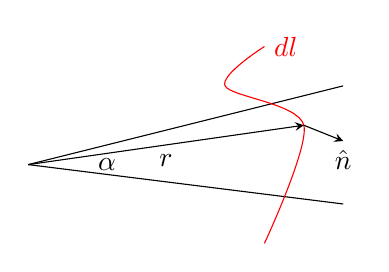
\begin{tikzpicture}
		
		\draw[color=black] (0,0) -- (4, 1);
		\draw [color=black] (0,0) -- (4,-0.5);
		
		\coordinate (A) at (1,0);
		\node at (A) {$\alpha$};
		
		\draw [red] plot [smooth] coordinates {(3, -1) (3.5, 0.5) (2.5, 1) (3, 1.5)} node [right] {$dl$};
		\draw  [-stealth] (3.5,0.5) -- (4, 0.3) node [below] {$\hat{n}$};
		\draw[-stealth] (0,0) -- (3.5,0.5) node [midway, below] {$r$};
		
	\end{tikzpicture}
\caption{Angolo Piano}
\end{figure}

Sappiamo che tale angolo è dato da $d\alpha = \frac{dl}{r}$, dove $dl$ è un arco di circonferenza ma che può sempre essere considerata come una curva generica con una propria normale. In questo caso più generale avremo che $d\alpha = \frac{\hat{r} \cdot \hat{n} dl}{r}$. L'integrale di questo angolo piano in tutto il dominio in cui sia possibile integrarlo vale $2\pi$.

Passando quindi alle 3 dimensioni definiamo l'angolo solido: 
\begin{figure}[ht]
	\centering
	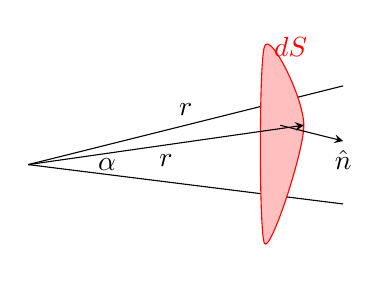
\begin{tikzpicture}
		
		\draw[color=black] (0,0) -- (4, 1) node [midway, above] {$r$};
		\draw [color=black] (0,0) -- (4,-0.5);
		
		\coordinate (A) at (1,0);
		\node at (A) {$\alpha$};
		
		\draw[red, fill=red!25] plot [smooth cycle] coordinates {(3, -1) (3.5, 0.5)  (3, 1.5)} node [right] {$dS$};
		\draw  [-stealth] (3.2,0.5) -- (4, 0.3) node [below] {$\hat{n}$};
		\draw[-stealth] (0,0) -- (3.5,0.5) node [midway, below] {$r$};
		
	\end{tikzpicture}
	\caption{Angolo Solido}
\end{figure}

In questo caso avremo dunque: 

\begin{equation}
	d\Omega = \frac{\hat{r} \cdot \hat{n} dS}{r^2}
\end{equation}

E il massimo angolo solido ottenibile integrando in tutto il dominio andrà a stagliare una sfera, il cui angolo solido è $4\pi$. 

\subsection{Flusso del campo elettrostatico}
Sia il campo vettoriale $\vec{E}$ preso un elemento di superficie $dS$ infinitesimo, caratterizzato dalla sua normale: 

\begin{figure}[ht]
	\centering
	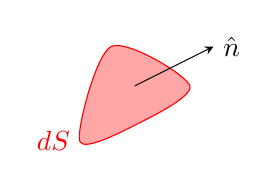
\begin{tikzpicture}
		\draw[red, fill=red!35] plot [smooth cycle] coordinates {(0,0) (0.7,0.5) (-0.3, 1) (-0.7, -0.2)} node [left] {$dS$};
		\draw[-stealth] (0,0.5) -- (1,1) node [right] {$\hat{n}$};
	\end{tikzpicture}
\end{figure}

Definiamo \textbf{flusso del campo $\vec{E}$} il valore: 

\begin{large}
	\begin{equation} \label{eq_flusso}
		d\Phi = \vec{E} \cdot d\vec{S} \rightarrow \Phi(\vec{E}) = \int_{S} \vec{E} \cdot d\vec{S} 
	\end{equation}
\end{large}

dove $d\vec{S} = dS\hat{n}$. L'unità di misura è $\left[ Vm^2/m =  Vm\right]$, stiamo parlando di una quantità \textbf{scalare}. 

\subsection{Enunciato del Teorema}
Il teorema che andremo a presentare di seguito ci dice che il flusso di $\vec{E}$ attraverso una \textbf{qualsiasi superficie chiusa} è uguale al rapporto tra la somma delle \textbf{cariche interne alla superficie} e il coefficiente $\epsilon_0$. 

\begin{tcolorbox}[colframe=red, colback=red!10, title=Teorema di Gauss]
	\begin{large}
		\begin{equation}
			\Phi (\vec{E}) = \oint_S{\vec{E} \cdot d\vec{S}} = \frac{Q_{tot}}{\epsilon_0}
		\end{equation}
	\end{large}
\end{tcolorbox}
 
\medskip
Questo teorema è anche noto come \textbf{2° Equazione di Maxwell} . Si noti quindi come il flusso del campo non sia dipendente dalla distanza dalla sorgente della carica. 

Andiamo ora ad analizzare il contributo che porta una carica esterna alla superficie presa in considerazione: 
in particolare all'interno di una superficie chiusa, per ogni elemento di superficie $dS$ ne avremo sempre uno dalla parte opposta con normale diretta in direzione opposta.

 Ciò porta ad avere da un lato flusso di modulo uguale, che da una parte è positivo, dall'altra è negativo. Dato che i contributi delle varie cariche si sommano, arriviamo a dire che le \textbf{cariche esterne} alla superficie di Gauss sono totalmente \textbf{ininfluenti}.

\begin{tcolorbox}
	\centering
	Le sorgenti di $\vec{E}$ sono le \textbf{singole cariche}
\end{tcolorbox}

Si può notare, tracciando il grafico del campo in funzione della distanza dalle sorgenti, che a volte il campo può presentare una \textbf{discontinuità} data dal valore $\Delta E = \frac{\sigma}{\epsilon_0}$, questo accade nel momento in cui il campo deve attraversare una superficie carica $\sigma$ e accade \textit{sempre}, si può dimostrare mediante l'utilizzo del teorema di Gauss.

\paragraph{Calcolo del campo di due piani indefiniti}

Vediamo ora il calcolo del campo per due piani indefiniti. Un calcolo che tornerà molto utile una volta introdotti i \textbf{condensatori}.

\begin{figure}[ht]
	\centering
	\begin{tikzpicture}
		\draw (0,0) -- (0,0.1) -- (10,0.1) -- (10, 0) -- (0,0) node [midway, above] {$\sigma^+$};;
		\draw[stealth-stealth] (-1, 0) -- (-1,-2) node [midway, left] {$h$};
		\draw (0,-2) -- (0,-2.1) -- (10,-2.1) -- (10, -2) -- (0,-2) node [midway, below] {$\sigma^-$};;
	\end{tikzpicture}
	\caption{Sovrapposizione di piani indefiniti}
\end{figure}

Effettueremo questo calcolo tramite il principio di \textbf{sovrapposizione}.  Il campo risultante sarà dunque dato dalla somma trai campi generato dal piano $\sigma^+$ e dal piano $\sigma^-$. Sappiamo anche che dato un piano indefinito il suo campo è dato da

\begin{equation} \label{eq_campo_piano_indefinito}
	\vec{E}(r) = \frac{\sigma}{2\epsilon_0} = \begin{cases}
		+ \frac{\sigma}{2\epsilon_0}  &  \text{se } z > 0 \\
		- \frac{\sigma}{2\epsilon_0} & \text{se } z < 0
	\end{cases}
\end{equation}

È facile immaginare a questo punto come all'esterno dei due piani il campo sia nullo e che internamente il campo sarà la somma dei due campi. La direzione sarà certamente quella dalla distribuzione positiva a quella negativa. Dunque avremo: 

\begin{equation} \label{eq_campo_condensatore}
	\vec{E}(r) = \frac{\sigma}{\epsilon_0}
\end{equation}

Si noti come la distanza \textbf{h non influisce nel calcolo del campo}

\section{Elettrostatica nei Conduttori}

Nel momento in cui andiamo ad accendere un campo, ogni carica presente nei materiali sente questo campo. In natura possiamo osservare due situazioni principali: 

\begin{itemize}
	\item \textbf{cariche libere}: l'esempio classico è quello del metallo, in questa situazione essendo le cariche libere di muoversi, verrà a generarsi un nuovo campo, dato dalla ridistribuzione della carica. 
	\item \textbf{dielettrici}: in questo genere di materiale le cariche sono fortemente vincolate agli atomi.
\end{itemize}

\subsection{Proprietà dei Conduttori in Equilibrio}

\begin{figure} [ht]\label{fig_conduttore}
	\centering
	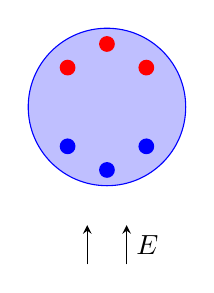
\begin{tikzpicture}
		\draw[color=blue, fill=blue!25] (0,0) circle [radius=1];
		\draw[-stealth] (0.25,-2) -- (0.25,-1.5) node [midway,right] {$E$};
		\draw[-stealth] (-0.25,-2) -- (-0.25,-1.5);
		
		\fill[color = red] (0,0.8) circle [radius=0.1];
		\fill[color = red] (0.5,0.5) circle [radius=0.1];
		\fill[color = red] (-0.5,0.5) circle [radius=0.1];
		
		\fill[color = blue] (0,-0.8) circle [radius=0.1];
		\fill[color = blue] (0.5,-0.5) circle [radius=0.1];
		\fill[color = blue] (-0.5,-0.5) circle [radius=0.1];
	\end{tikzpicture}
\caption{Conduttore in presenza di un Campo Esterno}
\end{figure}

\begin{itemize}
		\item le cariche positive sentiranno una forza lungo la direzione del campo, mentre le cariche negative sentiranno tale forza in direzione opposta a quella del campo
		
		\item la separazione di cariche va ad \textbf{indurre un campo} al quale si sovrappone il campo esterno. All'interno in questo modo avremo due contributi: $E_{indotto} + E_{esterno}$
		
		\item in un conduttore all'equilibrio il \textbf{campo interno è nullo}. Se non fosse nullo, gli elettroni sarebbero in moto
		
		\item nel momento in cui ho campo interno nullo, per ogni curva da un punto $A$ a $B$ il lavoro è sempre nullo. Ciò implica che anche il \textbf{potenziale sarà costante}, in particolare tale potenziale sarà quello della superficie.
		
		\item dal momento in cui il campo è nullo, per il Teorema di Gauss, avrò carica interna nulla, avrò quindi soltanto \textbf{cariche distribuite sulla superficie del conduttore}. 
		
		\item il campo della superficie del conduttori è dato da $\frac{\sigma}{\epsilon_0} \hat{n}$, questo è il \textbf{Teorema di Coulomb}. Tale campo è \textbf{normale alla superficie}
\end{itemize}

\subsection{Cavità in un Conduttore}
Ora che siamo riusciti ad osservare le proprietà dei conduttori, ci interessa comprendere che cosa succede nel momento in cui all'interno del conduttore in questione andiamo ad inserire una cavità vuota. 

Ipotizziamo di avvicinare una carica al nostro conduttore, questo tipo di struttura ha l'importante caratteristica di mantenere una densità di carica sulla superficie della cavità e un campo interno alla cavità \textbf{nulli}. 

Questi due fatti si possono ricavare tramite il teorema di Gauss. Dato che siamo in presenza di un conduttore, sappiamo che internamente al conduttore abbiamo campo nullo, e applicando il teorema di Gauss (utilizzando una superficie gaussiana adiacente alla cavità)otteniamo: $\oint Eds = 0 = Q_{int} / \epsilon_0 \rightarrow Q_{int} = 0$. 

Sappiamo anche che il campo elettrostatico è un campo conservativo, questo ci dice che la circuitazione lungo un cammino chiuso deve essere nulla. L'unico modo perché questo fatto sia vero, il campo interno alla cavità \textbf{deve} essere nullo, altrimenti avremmo circuitazione $\ne$ 0. Questo ci dice che non è possibile avere una separazione di carica per mantenere nulla la carica interna alla cavità.

Avendo campo nullo, all'interno della cavità il \textbf{potenziale è lo stesso del potenziale iniziale}. Questo significa che la differenza di potenziale tra il dentro ed il fuori rimane \textit{costante}, ciò vuol dire che l'informazione, non essendoci variazioni nelle differenze di potenziale, non viene mai trasmessa all'interno dello \textbf{schermo elettrostatico}. 

\section{Capacità Elettrostatica}
Si tratta di una proprietà che va a riguardare \textbf{conduttori isolati} e \textbf{condensatori}. Abbiamo visto che una certa distribuzione di cariche questa genera un \textbf{campo}, al quale è possibile associare un \textbf{potenziale}, si veda \ref{eq_potenziale_puntiforme} dalla quale possiamo ricavare che il potenziale è \textbf{lineare nella carica}. 

\subsection{Conduttore Isolato}

Consideriamo un conduttore che sia isolato elettrostaticamente e ipotizziamo di caricare tale conduttore con una carica $Q$. In questo momento la carica si distribuisce su tutta la superficie del conduttore e questo va ad un certo potenziale costante.

Definiamo \textbf{capacità} $C$ nel modo seguente: 

\begin{large}
	\begin{equation} \label{eq_cap_cond_isolato}
		C \coloneqq \frac{Q}{V}   \; \;\;\left[ F\right]
	\end{equation}
\end{large}

Si consideri che questa capacità è una proprietà che dipende unicamente dalla \textit{geometria} del sistema che andiamo a considerare e dal mezzo ($\epsilon_0$) in cui questo conduttore è immerso.

Si consideri ad esempio una sfera isolata di raggio $R$. Sottoposta ad una carica $Q$ questa sfera andrà a potenziale $Q/(4\pi\epsilon_0 R)$.Da cui avremo $C = 4\pi\epsilon_0R$. 

\subsection{Condensatore}
Si tratta in sostanza di un conduttore non isolato: ipotizziamo che dati due conduttori, una carica $Q$ del conduttore $C_1$ venga spostata al conduttore $C_2$. Ciò implica che su $C_1$ andrà a comparire una $-Q$. In questo modo $C_2$ andrà al potenziale $V2$ e $C_1$ andrà a $V_1$. Immaginiamo ora di avvicinare i due conduttori, in particolare $C_1$ sentirà il campo generato da $C_2$ e viceversa. 

In realtà in un sistema non isolato sono presenti conduttori in grande quantità, basti banalmente pensare alla Terra. Per semplificare il nostro operato ipotizzeremo di lavorare in condizioni di \textbf{induzione completa}. In pratica andremo ad allontanare gli altri conduttori in esame verso l'infinito, in modo che il loro effetto sia trascurabile.  Per ottenere induzione completa abbiamo a disposizione diverse strade:

\begin{itemize}
	\item mettiamo uno dei due conduttori all'interno nella cavità dell'altro conduttore La capacità è data da $\frac{Q}{\Delta V}$. Notare che allontanando l'armatura del conduttore più esterno all'infinito otteniamo di nuovo il caso del conduttore isolato. L'applicazione di ciò è data dal \textbf{condensatore sferico} che presenta \textit{induzione completa ideale}.
	
	\item \textbf{struttura tubolare} nella quale la lunghezza è molto maggiore rispetto alla sezione. Alla metà del tubo siamo chiaramente in una situazione di cavità. L'applicazione pratica di ciò  è il \textbf{condensatore cilindrico},
	
	\item \textbf{due lamine affiancate} in cui le superfici siano molto maggiori della distanza tra le lamine. Questa situazione si può approssimare ad un \textbf{condensatore piano}.
\end{itemize}

\subsection{Collegamento di Condensatori}
Per aumentare la capacità di un sistema abbiamo a disposizione due modi di collegare tra di loro i condensatori: in \textbf{serie} oppure in \textbf{parallelo}

\paragraph{Collegamento in Serie} Si tratta di un collegamento di $n$ condensatori che ha la caratteristica di avere la \textit{stessa carica nelle armature}, nel quale il potenziale totale è dato dalla \textit{somma} dei singoli potenziali.

\begin{figure}[ht]
	\centering
	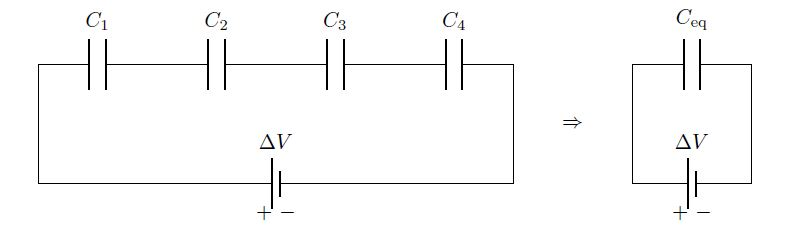
\includegraphics[width=0.7\linewidth]{Media/condensatori_serie}
	\caption {Collegamento di capacitori in serie}
	\label{fig:condensatoriserie}
\end{figure}

In questo caso, ricordando che la capacità è data da \ref{eq_cap_cond_isolato}, avremo

\begin{large}
	\begin{equation} \label{eq_cap_serie}
		C_{tot} \coloneqq \frac{Q}{\sum_{i}  \frac{Q}{C_i}} \; \rightarrow \frac{1}{C_{tot}} = \sum_{i=1}^{n} \frac{1}{C_i}
	\end{equation}
\end{large}

Notiamo quindi che il collegamento in serie serve a \textbf{ridurre} la capacità totale a parità di potenziale.


\paragraph{Collegamento in Parallelo}
Si tratta di un collegamento che ha la caratteristica di avere lo \textbf{stesso potenziale}.

\begin{figure}[H]
	\centering
	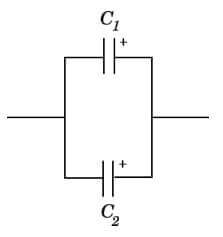
\includegraphics[width=0.5\linewidth]{Media/condensatoriparallelo}
	\caption{Collegamento di capacitori in parallelo}
	\label{fig:condensatoriparallelo}
\end{figure}


In questo caso, considerando che la carica sarà data dalla somma delle cariche dei singoli capacitori avremo: 

\begin{large}
	\begin{equation} \label{eq_cap_parallelo}
		Q_{tot} = \sum_{I}  C_i V_i \rightarrow C_{tot} \coloneqq \sum_{i} C_i
	\end{equation}
\end{large}

\paragraph{Partitore Capacitivo}
Si tratta di un elemento tipico di molti circuiti elettrici. È un collegamento di condensatori in serie nel quale si richiede di calcolare come si ripartisce il potenziale collegato agli estremi nei vari elementi del circuito. 

\begin{figure}[ht]
	\centering
	\begin{tikzpicture}
		\draw (-1,0) -- (0,0) (0.5,0) -- (1.5,0) (2,0) -- (3,0) (3.5,0) --(4.5,0);
		\draw (0,0.25) -- (0,-0.25) (0.5,0.25) -- (0.5, -0.25) (1.5,0.25) -- (1.5,-0.25) (2,0.25) -- (2, -0.25) (3,0.25) -- (3,-0.25) (3.5,0.25) -- (3.5, -0.25);
		
		\node at (0.25, -0.5) {$C_1$};
		\node at (3.25, -0.5) {$C_n$};
		\node at(-0.2,0.5) {$Q$};
		\node at (0.8,0.5) {$-Q$};
	\end{tikzpicture}
\end{figure}

Sapendo che su ogni capacitore è presente lo stesso valore di $Q$ avremo che $V_i = \frac{Q}{C_i}$. Sappiamo anche che $Q = C_{tot}V_{tot}$, dunque avremo: 

$$ 
V_i = \frac{C_{tot}}{C_i} V_{tot}
$$

\subsection{Energia Immagazzinata nel Capacitore}
Vogliamo andare a trovare l'energia immagazzinata nel capacitore per poi provare a generalizzare il concetto trattando la \textbf{densità di energia elettrostatica}. Ipotizziamo di caricare le due armature del condensatore, spostando da un'armatura all'altra delle cariche positive. Ci troviamo nella seguente situazione: 

\begin{itemize}
	\item lo spostamento della prima carica $q_0$ avviene in modo gratuito, tale carica andrà a generare un \textbf{campo}
	
	\item spostare $q_2$ implica di fare lavoro contro il campo generato da $q_1$
\end{itemize}

Per ogni carica spostata compierò un lavoro espresso come

$$
dL_{est} = dqV(q)
$$

Il potenziale nella formula di cui sopra varia in base alla quantità di carica che viene depositata. Il lavoro per caricare il condensatore sarà dunque dato da

\begin{large}
	\begin{equation}
		L_{est} = \int_{0}^{Q} V(q) dq
	\end{equation}
\end{large}

Ma noi sappiamo che $V(q)$ è dato da $q/C$, dunque abbiamo: 

\begin{large}
	\begin{equation}
		U = \int_{0}^{q}\frac{q}{C} dq = \frac{1}{2} \frac{Q^2}{C} = \frac{1}{2} CV^2= \frac{1}{2} QV
	\end{equation}
\end{large}

Questa formula esprime l'\textbf{energia immagazzinata nel condensatore}. Utilizzando il campo del condensatore piano, possiamo esprimere la nostra energia come: 

\begin{large}
	\begin{equation}
		U = \frac{\epsilon_0}{2} E^2 \Sigma h
	\end{equation}
\end{large}

Dove $\Sigma h$ è il \textbf{volume} del condensatore piano, o meglio, il volume interno al condensatore nel quale abbiamo \textbf{campo non nullo}. Possiamo definire la \textbf{densità di energia} come: 

\begin{large}
	\begin{equation} \label{eq_densita_energia}
		\mu_E = \frac{\epsilon_0 E^2}{2} \;\;\;  \left[  \frac{J}{m^3} \right]
	\end{equation}
\end{large}

\section{Elettrostatica nei Dielettrici}

Questi materiali sono caratterizzati dal fatto che si compongono di \textbf{cariche vincolate all'atomo}. Nel momento in cui viene acceso un campo esterno attorno al dielettrico, il centro delle cariche positive si sposta lungo la direzione del campo, mentre quello delle cariche negative si sposta in direzione opposta, questo a motivo del fatto che vale la legge di Coulomb \ref{f_coulomb}. In questo modo viene a formarsi un \textbf{dipolo elettrico}

\begin{figure} [ht]
	\centering
	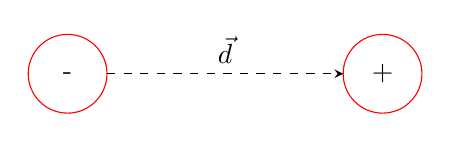
\begin{tikzpicture}
		\draw [color = red] (-2,0) circle [radius = 0.5]; 
		\draw[color=red] (2,0) circle [radius=0.5];
		
		\node at (-2,0) {-};
		\node at (2,0) {+};
		
		\draw[dashed, -stealth] (-1.5,0) -- (1.5,0) node [midway , above] {$\vec{d}$};
	\end{tikzpicture}
\caption{Dipolo Elettrico}
\end{figure}

Definiamo il \textbf{dipolo elettrico} un sistema di due carica, con segno opposto e modulo uguale, che rimangono vincolate ad una distanza fissa $d$. 

Definiamo il \textbf{momento di dipolo} come il prodotto tra cariche e distanza: 

\begin{large}
	\begin{equation} \label{eq_momento_dipolo}
		\vec{p} \coloneqq q\vec{d}
	\end{equation}
\end{large}

Per ricordare il verso del vettore $d$ può essere utile notare che va nello stesso verso del campo.

Nel momento in cui si accende un campo attorno ad un isolante, abbiamo due situazioni che possono venirsi a creare: 

\begin{itemize}
	\item il materiale si \textbf{polarizza}, arrivando ad una separazione di carica. A differenza dei conduttori, il campo qui non è nullo
	
	\begin{figure}[th]
		\centering
		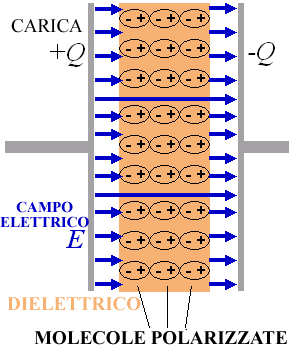
\includegraphics[width=0.5\linewidth]{Media/polarizzazione}
		\caption{Dielettrico Polarizzato}
		\label{fig:polarizzazione}
	\end{figure}
	
	\item il materiale potrebbe essere \textbf{già polarizzato} sebbene il momento di dipolo medio sia nullo. Nel momento in cui il campo esterno di accende, i dipoli sentono \textbf{momento meccanico} $\tau$ fino a quando i dipoli non saranno allineati al campo esterno. 
\end{itemize}

Ovviamente noi andremo a lavorare, non con i singoli dipoli ma con un \textbf{campo di polarizzazione} $\vec{P}(\vec{r})$ definito nel modo seguente: 

\subsection{Condensatore riempito di Dielettrico}
Ipotizziamo di avere un condensatore piano riempito di materiale dielettrico: 

\begin{figure} [H]
	\centering
	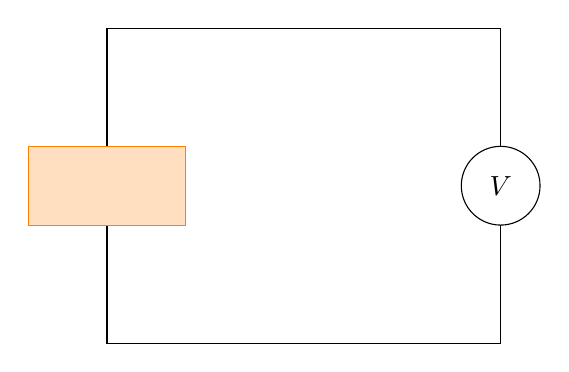
\begin{tikzpicture}
		\draw (0,3) -- (0,4.5) -- (5,4.5) -- (5,3);
		\draw (-1,3) -- (1,3) (-1, 2) -- (1,2);
		\draw (5, 2.5) circle [radius=0.5];
		\node at (5,2.5) {$V$};
		\draw (0,2) -- (0,0.5) -- (5,0.5) -- (5,2);
		
		\draw [color = orange, fill=orange!25] (-1,3) -- (1,3) -- (1,2) -- (-1,2) -- (-1,3);
	\end{tikzpicture}
\end{figure}

Sappiamo che nel \textbf{vuoto} la capacità del condensatore è data da $\frac{\epsilon_0 \Sigma}{d}$ e che $Q = C_0 V_0$, mentre $E_0 = \sigma_0 / \epsilon_0$, con $\Delta V = E_0 d$ .
Ipotizziamo ora di staccare il nostro sistema dal generatore, rimanendo dunque a carica costante, e di riempire di dielettrico il condensatore. 

Avremo che il potenziale del condensatore riempito di dielettrico sarà dato da: 

$$ 
V_k = \frac{V_0}{k}
$$

dove $k$ è detta \textbf{costante dielettrica del materiale}. Avendo un potenziale minore, avremo che la capacità del condensatore aumenta: 

$$
C_k = \frac{Q}{V} = kC_0 = k\epsilon_0 \frac{\sigma}{d}
$$

dove il valore $k\epsilon_0$ è detto \textbf{pernettività del materiale} (notare come $k_{vuoto} = 1$). Anche $E_k $ sarà scalato allo stesso modo del potenziale, in particolare sarà sempre non nullo, al contrario di quanto accade nel momento in cui riempiamo il condensatore di conduttore.

All'interno del dielettrico avremo un campo di indotto $E_p$ detto di polarizzazione che si oppone al campo $E_0$, questo è il motivo per cui il campo totale $E_k$ viene scalato di un certo fattore $k$. 
Le cariche più esterne relative ai dipoli si dicono \textbf{cariche di polarizzazione}.

\paragraph{Calcolo delle Cariche di Polarizzazione}
Vogliamo a questo punto andare a calcolare le cariche di polarizzazione nel nostro capacitore. Utilizzando il teorema di Gauss otteniamo che il campo totale all'interno del dielettrico è dato da: 

$$ 
E_{tot}= \frac{\left|\sigma_0\right|}{\epsilon_0} - \frac{\left|\sigma_p\right|}{\epsilon_0} 
$$

ma siccome abbiamo visto anche che $E_{tot} = \frac{E_0}{k}$ otteniamo un'espressione finale per le cariche di polarizzazione: 

\begin{large}
	\begin{equation} \label{eq_cariche_polarizzazione}
		\sigma_p = \sigma_0 \frac{k-1}{k}
	\end{equation}
\end{large}

La \textbf{polarizzazione} $\vec{P}(\vec{r})$ sarà data proprio da
\begin{large}
	\begin{equation}
		\left|\vec{P}\right| = \sigma_p
	\end{equation}
\end{large}

Dunque, dato un campo di polarizzazione potremo esprimere in un nuovo modo la $\sigma_p$: 
\begin{large}
	\begin{equation}
		\sigma_p^\pm = \vec{P} \cdot \hat{n}
	\end{equation}
\end{large}

\subsection{Dielettrici Lineari}
Definiamo un \textbf{dielettrico lineare} un dielettrico per il quale, nel momento in cui si accende il campo, la \textbf{polarizzazione è parallela e proporzionale al campo E}: 

\begin{large}
	\begin{equation} \label{eq_polarizzazione_lineare}
		\vec{P} = \epsilon_0 \chi \vec{E}
	\end{equation}
\end{large}

In questo caso il valore $\chi$ è detto \textbf{suscettività dielettrica del materiale}. Osservando l'equazione che ci dà $E_k = E_0 / k$, utilizzando $1 + \chi = k$ possiamo scrivere: 

$$ E_k = \frac{E_0}{1 + \chi} $$ 

\subsection{Teorema di Gauss per i Dielettrici}

Immaginiamo di avere un condensatore piano riempito di dielettrico, le cui cariche libere nella lastra superiore sono positive, viene da sé che le cariche di polarizzazione saranno negative. Utilizziamo come superficie di Gauss un cilindro con la base superiore nella lastra superiore. Applicando il teorema avremo

$$
\oint E = E_{cond}A_{base}  + E_{diel}A_{base} = \frac{\sigma_{libere}  - \sigma_{pol}}{\epsilon_0} A_{base}
$$

Avendo un conduttore, il valore di $E_{cond}$ è chiaramente nullo. Sappiamo anche che $\sigma_p = \vec{P} \cdot \hat{n}$ , ma tale valore è anche uguale a $d\Phi(P)$. Ottengo dunque: 

$$
\oint E \cdot dS = 	\frac{q_{lib}}{\epsilon_0} - \frac{ \oint \vec{P} \cdot d\vec{S}}{\epsilon_0}
$$

Vogliamo però ottenere un teorema che ci permetta di conoscere informazioni sulle sole cariche libere. Per fare ciò facciamo nel seguente modo: 

$$
\oint  \left(\epsilon_0 \vec{E} + \vec{P} \right) \cdot dS = Q_{libere}
$$

e, definendo $\vec{D} = \epsilon_0\vec{E}+ \vec{P}$ come \textbf{campo di induzione elettrica} otteniamo

\begin{tcolorbox}[colframe=red, colback=red!10, title=Teorema di Gauss nei Dielettrici]
	\begin{large}
		\begin{equation}
			\oint \vec{D} \cdot dS = Q_{libere}
		\end{equation}
	\end{large}
\end{tcolorbox}

\subsection{Riassunto}
Riassumendo quanto visto fino a qui sui dielettrici, possiamo concludere che date delle cariche sorgenti immerse in un dielettrico, verrà a generarsi un campo $E_{tot}$ dato dalla somma tra il campo iniziale e il campo di polarizzazione. Per ricavare informazioni andrò in primo luogo a calcolare $\vec{D} = \epsilon_0\vec{E} + \vec{P}$, dove $\vec{P} = \epsilon_0 \chi E$ 

Grazie alla costante dielettrica nota, posso a questo punto ricavare tutto ciò di cui ho bisogno come segue: 

\begin{itemize}
		\item $ \vec{D} = \epsilon_0 k \vec{E}_k  \longrightarrow \vec{E}_k= \frac{\vec{D}}{\epsilon_0k}$
		\item $\vec{P} = \epsilon_0 (k-1) \vec{E}$ oppure $\vec{P} = \frac{k-1}{k} \vec{D}$
		\item $\sigma_p (r=R) = \vec{P}(r=R)$
\end{itemize}

\section{Energia Elettrostatica}

Data una carica immersa in un campo elettrostatico, sappiamo che su tale carica agisce una forza descritta da \ref{f_coulomb} che vista in termini di campo diventa semplicemente $F = qE$. Sotto l'effetto di tale forza di Coulomb, che è \textit{conservativa}, entriamo nel mondo della dinamica. 

Alla luce della conservatività di questa forza, abbiamo modo di calcolare il lavoro di tale forza, ovvero

$$L_{elettr.} = -\Delta U_{elettr}$$

Se andiamo a porre l'energia all'infinito uguale a 0, possiamo riscrivere la formula del lavoro nel modo seguente: 

$$
L_{elettr.} = -q\Delta V
$$

Abbiamo visto come l'energia, nel caso in cui $U_{\infty} = 0$, rappresenta il \textbf{lavoro esterno necessario a costruire il sistema}, ma anche il \textbf{lavoro del campo per disassemblare il sistema} (portare tutte le cariche all'infinito).

\subsection{Distribuzione discreta di cariche}
Data una distribuzione discreta di cariche $\left\{q_i\right\}_{i:1...n}$ consideriamo il lavoro esterno necessario alla costruzione del sistema, che corrisponderà all'energia immagazzinata nel sistema di cariche: 

\begin{itemize}
	\item  porto $q_1$ da $\infty$, non avendo forze in gioco, compio $L_1 = 0$
	\item  porto $q_2$ da $\infty$, sento in questo momento il campo generato da $q_1$: $L_2 = q_2V_1(r_2) \; = \; q_2\frac{q_1}{4\pi\epsilon_0r=r_2}$
	\item ...
	\item per quanto riguarda la $n-$esima carica, sfrutteremo il principio di sovrapposizione: $L_n = q_n (\Delta V_{tot}) \; = \; q_n(V_1(r_n) + ... + V_i(r_n) + ... V_{n-1}(r_n))$ 
\end{itemize}

Per la particella $i-$esima il potenziale sarà dato da: 

$$
\frac{q_i}{4\pi\epsilon_0r=r_n}
$$

Il lavoro totale sarà quindi dato dalla somma di tutte le componenti appena descritte, e quindi l'energia sarà data da: 

\begin{large}
	\begin{equation} \label{eq_energia_sistema_discreto}
		U_{el} = \frac{1}{2} \sum_i^n q_iV_i \; = \;  \frac{1}{2}\sum_i ^n\sum_{j \ne i}\frac{q_j}{4\pi\epsilon_0r_{ij}}
	\end{equation}
\end{large}

\subsection{Distribuzione continua di cariche}
Andiamo ora a generalizzare quanto visto fino a questo momento per la distribuzione \textbf{continua} di cariche. È abbastanza intuitivo capire che per passare al continuo le sommatorie dovranno diventare degli \textit{integrali} nello spazio. 

Dati dunque due volumetti unitari, rispettivamente a distanza $r_1$ ed $r_2$ dall'origine degli assi, ciascuno del volume $d\tau_1, d\tau_2$ a distanza, l'uno dall'altro $r_{12}$; avremo che per portare il primo volumetto, non compieremo lavoro, per quanto riguarda invece il secondo compieremo un certo lavoro, espresso dall'energia unitaria che segue: 

$$
dU_{el} = \frac{\rho (r_1) d\tau_1\rho(r_2)d\tau_2}{4\pi\epsilon_0r_{12}}
$$

dove $\rho d\tau_1$ corrisponde a $dq_1$, lo stesso vale per $dq_2$, possiamo a questo punto passare all'energia totale: 

\begin{large}
	\begin{equation} \label{eq_energia_sistema_continuo}
		U_{el} = \frac{1}{2} \frac{\int_{vol}\int_{vol} \rho(r_1) \rho(r_2)}{4\pi\epsilon_0r_{12}} d\tau_1 d\tau_2
	\end{equation}
\end{large}

tramite le opportune semplificazioni, otteniamo: 

\begin{large}
	\begin{equation} \label{eq_energia_sistema_continuo_semplificata}
		\frac{1}{2} \int_{vol} \rho(r) V(r) d\tau
	\end{equation}
\end{large}

\subsection{Sistema di conduttori}
Ipotizziamo ora di essere in un sistema di conduttori, nei quali ricordando quanto già visto, abbiamo carica distribuita unicamente in superficie, e potenziale costante. A questo punto potremo utilizzare \ref{eq_energia_sistema_continuo_semplificata}. Data infatti la carica: 

$$ Q_i = \int_{sup} \sigma_i dS $$ 

otteniamo

$$
	U_{el} = \frac{1}{2} \int \rho V d\tau \; = \; \frac{1}{2} \sum_{i=1}^n \int_{sup} \sigma_i V_i
$$

e, dato che il potenziale è costante, possiamo scrivere

\begin{equation} \label{eq_energia_sistema_conduttori}
	U_{el} = \frac{1}{2} \sum_{i=1}{n} Q_i V_i
\end{equation}

Rispetto all'equazione \ref{eq_energia_sistema_discreto}, nella quale $V_i$ rappresenta il potenziale di interazione, dunque soltanto quello delle \textbf{altre cariche}, in questa equazione il potenziale rappresenta anche il \textbf{lavoro necessario a caricare il singolo conduttore}, questo a motivo del fatto che, sebbene il primo conduttore venga caricato gratuitamente, avvicinando il secondo conduttore al sistema, questo sente induzione dovuta al primo. Questo lavoro in pratica comprende sia il lavoro di interazione, che il lavoro di carica del conduttore stesso.

\paragraph{Due conduttori in induzione completa} Ipotizziamo ora di avere due conduttori, il primo caricato a $Q_1$ e a potenziale $V_1$, il secondo con $Q_2, V_2$. Applicando quanto visto in precedenza avremo che: 

$$ U_{el} = \frac{1}{2} \sum_1^2 Q_iV_i = \frac{1}{2} \left(Q_1V_1 + Q_2V_2\right) $$

Sappiamo che, avendo un \textbf{condensatore} (conduttori in induzione completa), avremo $Q_1 = C(V_1 - V_2)$ e $Q_2 = -Q_1$. Inserendo quanto appena visto nell'equazione di cui sopra otteniamo: 

$$U_{el} = \frac{1}{2}C\Delta V^2$$

\subsection{Densità di Energia Elettrostatica}
Andiamo ora a trattare l'energia elettrostatica immagazzinata all'interno del campo elettrostatico. È dimostrabile che il risultato ottenuto per il condensatore nell'equazione \ref{eq_densita_energia}, è in realtà un risultato che vale in \textbf{generale}. 

\section{Dipolo Elettrico}
In questa situazione abbiamo due cariche di segno opposto vincolate da una distanza rigida $d$, caratterizzato da un momento di dipolo $\vec{p} = q\vec{d}$. 

Vogliamo calcolare il potenziale del seguente sistema in un punto $P$: 

\begin{figure}[H]
	\centering
	\begin{tikzpicture}
		% assi cartesiani
		\draw[color=black!50, -stealth] (0,0) -- (0,3);
		\draw[color=black!50, -stealth] (0,0) -- (-2.5, -1.5);
		\draw[color=black!50, -stealth] (0,0) -- (2.5,-1.5);
		
		\fill[color=black] (0,1.5)  circle [radius=0.1] node [above] {$+q$};
		\fill[color=black] (0,-1.5)  circle [radius=0.1] node [above] {$-q$};
		
		\fill[color=black] (5,2)  circle [radius=0.1] node [above] {$P$};
		
		\draw[color=black,dashed] (0,1.5) -- (5,2) node [midway, above] {$r^+$};
		\draw[color=black,dashed] (0,-1.5) -- (5,2) node [midway, above] {$r^-$};
		\draw[color=red, dashed, -stealth] (0,0) --(5,2) node  [midway, above] {$r$};
						
		\draw[dashed, color=blue!50] (0,-1.5) -- (0,1.5) node [midway,left] {$d$};
	\end{tikzpicture}
\end{figure}


Il \textbf{potenziale} $V$ si calcolerà tramite principio di sovrapposizione ed è dato dalla somma dei potenziali delle due cariche : 

$$
V = V_+ + V_-  \; = \;  \frac{1}{4\pi\epsilon_0} \left(\frac{q}{r_+} - \frac{q}{r_-}\right) = \frac{q}{4\pi\epsilon_0} \frac{r_- - r_+}{r_+r_-}
$$

Considerando il fatto che stiamo utilizzando oggetti molto piccoli, basterà prendere il \textit{baricentro} del dipolo come punto di partenza dei due raggi vettori, posso in pratica effettuare una \textbf{approssimazione di punto lontano}, che mi permette di non andare a vedere la struttura di una struttura microscopica. 

Avremo quindi che $r_+r_-$ diventa $r^2$ e tramite la trigonometria $r_- - r_+$ diventa $dcos\theta$ dove $\theta$ è l'angolo tra la distanza rigida e il raggio vettore che collega al punto $P$.  
Ricordando che $qd = p \rightarrow q = p/d$ e che $a \cdot b = abcos\theta$, otteniamo

$$ 
V(\vec{r}) = \frac{\vec{p} \cdot \vec{r}}{4\pi\epsilon_0 r^3}
$$ 

Si noti come il potenziale del dipolo scende più rapidamente del potenziale della singola carica. Per arrivare a tale formula notiamo come la carica $q = p/d$ si semplifichi con $dcos\theta$ .


Vogliamo ora studiare il \textbf{campo} del dipolo elettrico, in particolare osservarne le linee di campo. Sappiamo che il potenziale è nullo nel momento in cui $\vec{p} \perp \vec{r}$. Sopra il piano avremo potenziale positivo, sotto avremo invece potenziale negativo. Sappiamo che il campo va dal potenziale positivo a quello negativo, e che le linee di campo sono sempre ortogonali alle superfici equipotenziali. Questo ci può dare un'idea chiara dell'andamento delle linee di campo.

\begin{figure}[H]
	\centering
	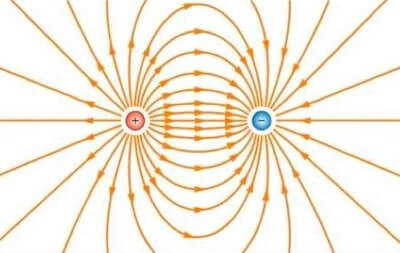
\includegraphics[width=0.5\linewidth]{Media/linee_campo_dipolo}
	\caption{Linee di Campo di un Dipolo}
	\label{fig:lineecampodipolo}
\end{figure}

\subsection{Dipolo Elettrico in un campo esterno costante}
%Immaginiamo di immergere il nostro dipolo elettrico all'interno di un campo esterno. Vogliamo studiare il comportamento di tale oggetto. Innanzitutto le due cariche di cui si compone il dipolo sentiranno una forza $\vec{F} = q\vec{E}$. Chiaramente, essendo le due cariche di segno opposto le forze saranno a verso opposto, la risultante sarà dunque nulla, e quindi il dipolo sarà impossibilitato a traslare. 

Tuttavia queste due forze costituiscono una coppia di forze applicate al polo, si verificherà dunque una \textbf{rotazione} a causa di un momento torcente $\vec{\tau} \ne 0$. Il valore di tale $\vec{\tau}$ ci è dato da: 

$$ 
\vec{\tau} = \left(\vec{r} \times \vec{F} \right) = \vec{d} \times \vec{F}  = \vec{d} \times q\vec{E}  = \vec{p}  \times \vec{E}
$$

L'ultima uguaglianza si ottiene chiaramente spostando il la carica a sinistra del prodotto vettoriale. Otteniamo quindi la seguente equazione che rappresenta il \textbf{momento meccanico} sul dipolo a \textbf{causa del campo esterno}: 

\begin{large}
	\begin{equation} \label{eq_tau_dipolo_in_campo_esterno}
		\vec{\tau} = \vec{p} \times \vec{E} 
	\end{equation}
\end{large}

In pratica succede che il dipolo si \textbf{allinea al campo esterno}. Cercando invece andare a studiare l'\textbf{energia} del sistema abbiamo che il lavoro torcente è dato dall'equazione seguente: 

$$ 
dL = (\tau d\Theta)  = p E sen\theta d\theta = d(-pEcos\theta)
$$

Da ciò ricaviamo che 

\begin{large}
	\begin{equation} \label{eq_energia_interazione_campo_dipolo}
		U = -\vec{p} \cdot \vec{E}
	\end{equation}
\end{large}

Questa equazione ci fornisce l'\textbf{energia di interazione del dipolo nel campo esterno}. In pratica abbiamo massima energia nel momento in cui abbiamo \textbf{equilibrio instabile}, viceversa nel momento in cui abbiamo energia minima abbiamo equilibrio \textbf{stabile}.

Nel momento in cui immergiamo un dipolo in un \textbf{campo non omogeneo},  avremo che le forze sentite dal dipolo saranno: 
  
$$
F_x = \vec{p} \cdot \nabla E_x
$$

\section{Equazioni di Maxwell per l'elettrostatica}

La prima equazione è quella relativa al fatto che il campo elettrostatico è conservativo: 

\begin{equation} \label{eq_maxwell_campo_conservativo}
	\oint_\Gamma \vec{E} \cdot d\vec{l} = 0
\end{equation}

La seconda è anche nota come il teorema di Gauss: 

\begin{equation}
	\oint_{sup} \vec{E} \cdot d\vec{S} = \frac{Q_{int}}{\epsilon_0}
\end{equation}

Il significato del teorema di Gauss è chiaramente quello che le sorgenti del campo sono unicamente le singole cariche. Quelle viste fino a questo momento sono le equazioni di Maxwell per l'elettrostatica e valgono a livello \textbf{macroscopico}. Abbiamo modo di ottenere queste formule che erano in \textbf{termini integrali} anche in \textbf{termini locali}, questo utilizzando il Teorema di Stokes ed il Teorema di Gauss della Divergenza. 


Le due equazioni di cui sopra in questo modo diventano, la prima tramite Stokes: 

$$
\nabla \times E = 0
$$

e, tramite la divergenza:

$$
\int_{vol} \nabla \cdot E d\tau = \frac{\rho}{\epsilon_0}
$$

Inoltre, abbiamo visto come $\Delta V = - \int_\gamma E \cdot dl$, tramite il teorema del gradiente possiamo scrivere la terza equazione locale per l'elettrostatica, considerando che $\Delta V = \int_\gamma \nabla V$: 

$$ \vec{E} = - \nabla V $$

e, utilizzando la seconda e la terza equazione, ricavare l'\textbf{equazione di Poisson} per l'elettrostatica: 

$$ \nabla^2 V = -\frac{\rho}{\epsilon_0} $$